\documentclass[a4paper,11pt,dvipdfmx]{ujarticle}
% パッケージ
\usepackage{graphicx}
\usepackage{url}
% レイアウト指定を記述したファイルの読み込み
\input{layout}

% タイトルと氏名を変更せよ．
\title{日本におけるデジタル化の状況}
\author{G684922026 本間 日咲}

\begin{document}

\maketitle %ここにタイ

\section{ブローバンドの整備状況}

OECDによるプロードバンド回線の普及に関する調査\cite{oecd}によると、図\ref{fig:加入率}に示すように、日本における 100人あたりのモバイルプロードバンドの加入者数は190.5で、第1位になっている。2位はエストニア
で、3位米国と続く。

\begin{figure}[htbp]
    \centering
    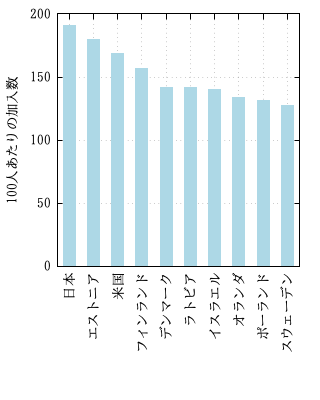
\includegraphics[scale=0.7]{fig21.png}
    \caption{光ファイバー線の加入者数（100人あたり）}\label{fig:加入率}
\end{figure}

\section{デジタル競争率ランキング}

際経営開発研究所（IMD）の調査\cite{imd}によると、日本のデジタル競争力のランキングは表\ref{tbl:デジタル競争率}に示すよ
うに、調査対象の64カ国中、総合で28位、技術分野で30位となっている。

\begin{table}[htbp]
    \centering
    \caption{デジタル競争率ランキング(64カ国中)}
    \label{tbl:デジタル競争率}

    \begin{tabular}{|c|c|c|}\hline
        国  & 総合 & 技術 \\
        \hline
        米国 & 1位 & 4位 \\
        \hline
        香港 & 2位 & 10位 \\
        \hline
        スウェーデン & 3位 & 8位 \\
        \hline
        デンマーク & 4位 & 2位 \\
        \hline
        シンガポール & 5位 & 3位 \\
        \hline
        \hline
        韓国 & 12位 & 13位 \\
        \hline 
        中国 & 15位 & 20位 \\
        \hline
        \hline
        日本 & 28位 & 30位 \\
        \hline
    \end{tabular}
\end{table}

\section{考察}

図\ref{fig:加入率}では、日本はプロードバンド回線の加入者数が多く、世界第1位であることから、通信インフラが充実しとぃることがわかる。
その一方で、表\ref{tbl:デジタル競争率}では、日本のデジタル競争力のランキングは64カ国中28位であり、技術分野でも30位であることから、通信インフラが充実しているにもかかわらず、デジタル競争力は低いことがわかる。
以上のことから、通信インフラの充実はデジタル競争力の向上に直結するわけではないことがわかる。
その理由として、デジタル競争力の向上には、通信インフラの充実だけでなく、技術革新やデジタル人材の育成などの要素も重要であると考える。
今後は通信インフラを整備するだけでなく、それを有効活用できる環境づくりが重要だと考える。


% ここから本文
% 節見出し: \section{}
% を使う

% 本文(1)
%  参考文献の参照: \cite{}
%  図番号の参照： \ref{}
% を使う
% 文献データベースのキーワードは oecd と imd
% になっている．

% 図の挿入
% \includegraphics{}
% を
% \begin{figure}[htbp]
% \end{figure}
% で囲み
% \caption{}
% で図のタイトルを入れる．
% \label{}
% を使って図番号が参照できるようにする
% また，
% \centering
% で図が中央に来るようにする

% ーーー
% 節見出し(2)

% 本文(2)

% 表の挿入
% \begin{tabular}
% \end{tabular}    
% による表の記述を 
% \begin{table}[htbp]
% \end{table}
% で囲み
% \caption{}
% で表のタイトルを入れる．
% \label{}
% を使って表番号が参照できるようにする
% また，
% \centering
% で表が中央に来るようにする

% ーーー
% 見出し(3)
% 考察
%
% \begin{itemize}
% \end{itemize}
% を使って箇条書きで記述する

% ここに参考文献が入る
%

\bibliographystyle{junsrt}
\bibliography{exercise.bib}

\end{document}